\chapter{Инженерная реализация}

\section{Описание реализации}

Выбранные архитектурные принципы, стандарты и инструменты, утверждённые на этапе проектирования, поддерживаются программной платформой Yii 2 Framework. Данная платформа ориентирована на ускорение процесса разработки web-проектов, в том числе API по принципу REST, за счёт наличия большого числа программных модулей и автоматической генерации программного кода на основе схем баз данных. В результате внутреннего проектирования предлагаемого решения выяснилось, что эта платформа является наиболее подходящей.

\subsection{Примеры запросов и ответов API}

Отправка запросов и получение ответов выполнялось с помощью среды тестирования и отладки API Postman. Каждое сообщение содержит заголовок и тело, содержимое которых определяется ресурсом в соответствии с диаграммой на рисунке \ref{uml:1}.
	
	Для отправки запроса на добавление здания необходимо передать API запрос, аналогичный представленному на рисунке \ref{query:buildings_post_to}. При этом возможны два сценария: здание успешно добавлено (рисунок \ref{query:buildings_post_from}), здание уже существует (рисунок \ref{query:buildings_post_err_exists}).

	\pagebreak

	\begin{figure}[t!]
		\centering
		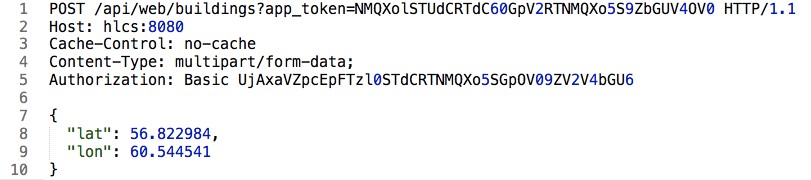
\includegraphics[width=0.8\textwidth]{images/queries/buildings_post_to}
		\caption{Пример запроса на добавление здания в САТУ}
		\label{query:buildings_post_to}
	\end{figure}

	\begin{figure}[t!]
		\centering
		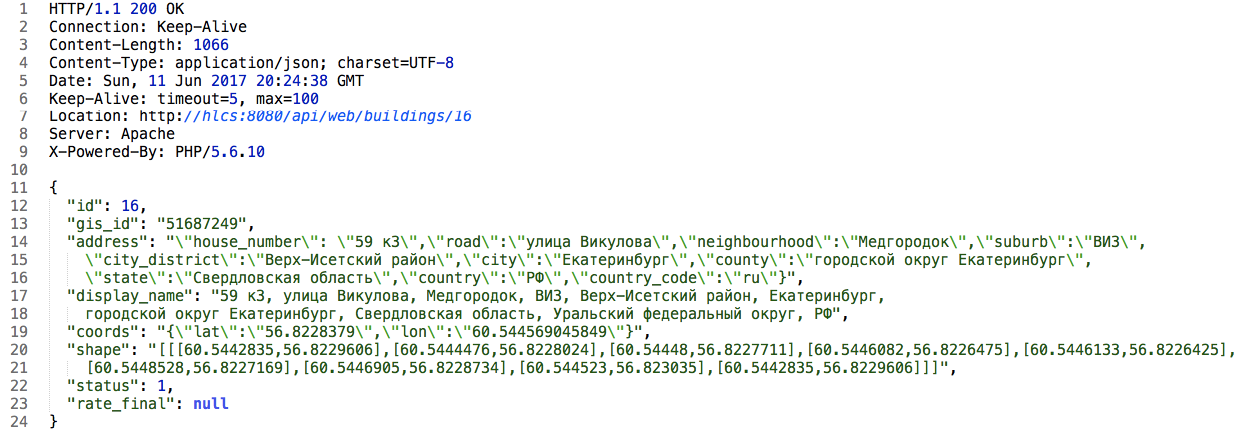
\includegraphics[width=1\textwidth]{images/queries/buildings_post_from}
		\caption{Успешный ответ к запросу на добавление здания в САТУ}
		\label{query:buildings_post_from}
	\end{figure}

	\begin{figure}[t!]
		\centering
		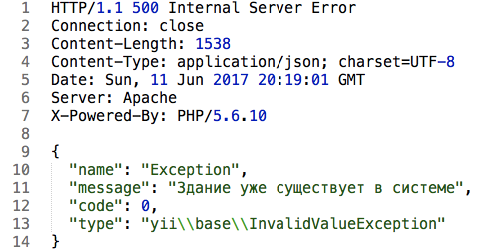
\includegraphics[width=0.5\textwidth]{images/queries/buildings_post_err_exists}
		\caption{Ответ к повторному запросу на добавление того же здания}
		\label{query:buildings_post_err_exists}
	\end{figure}

	Некоторые ресурсы требуют указания ключа авторизации. Если таковые отсутствуют, клиентскому приложению будет возвращён ответ, представленный на рисунке \ref{query:buildings_post_err_unauth}.

	\pagebreak

	\begin{figure}[t!]
		\centering
		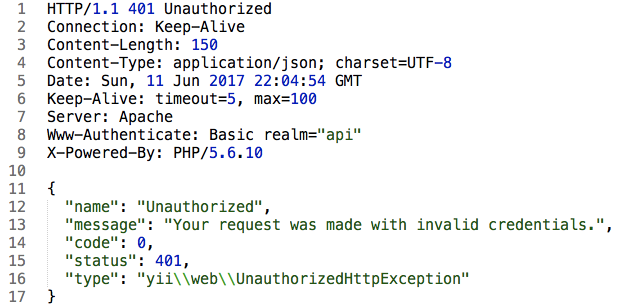
\includegraphics[width=0.6\textwidth]{images/queries/buildings_post_err_unauth}
		\caption{Ответ к запросу без ключа авторизации}
		\label{query:buildings_post_err_unauth}
	\end{figure}

	На рисунке \ref{query:buildings_get_to} приведен пример запроса на получение одной страницы списка всех зданий, соответствующий ответ - на рисунке \ref{query:buildings_get_from}. Из заголовка ответа видно, что объём каждой страницы - 20 элементов. При необходимости получить другую страницу следует изменить параметр \texttt{page}.

	\begin{figure}[t!]
		\centering
		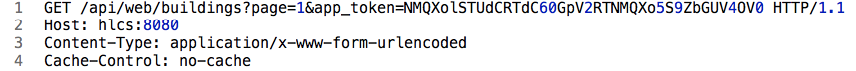
\includegraphics[width=0.9\textwidth]{images/queries/buildings_get_to}
		\caption{Пример запроса на получение списка зданий}
		\label{query:buildings_get_to}
	\end{figure}

	Если требуется получить информацию только по одному конкретному зданию, то к URI предыдущего запроса следует добавить идентификатор здания (рисунок \ref{query:buildings_get_one_to}). В результате от сервера API придёт ответ, аналогичный примеру на рисунке \ref{query:buildings_get_one_from}.

	\pagebreak

	\begin{figure}[t!]
		\centering
		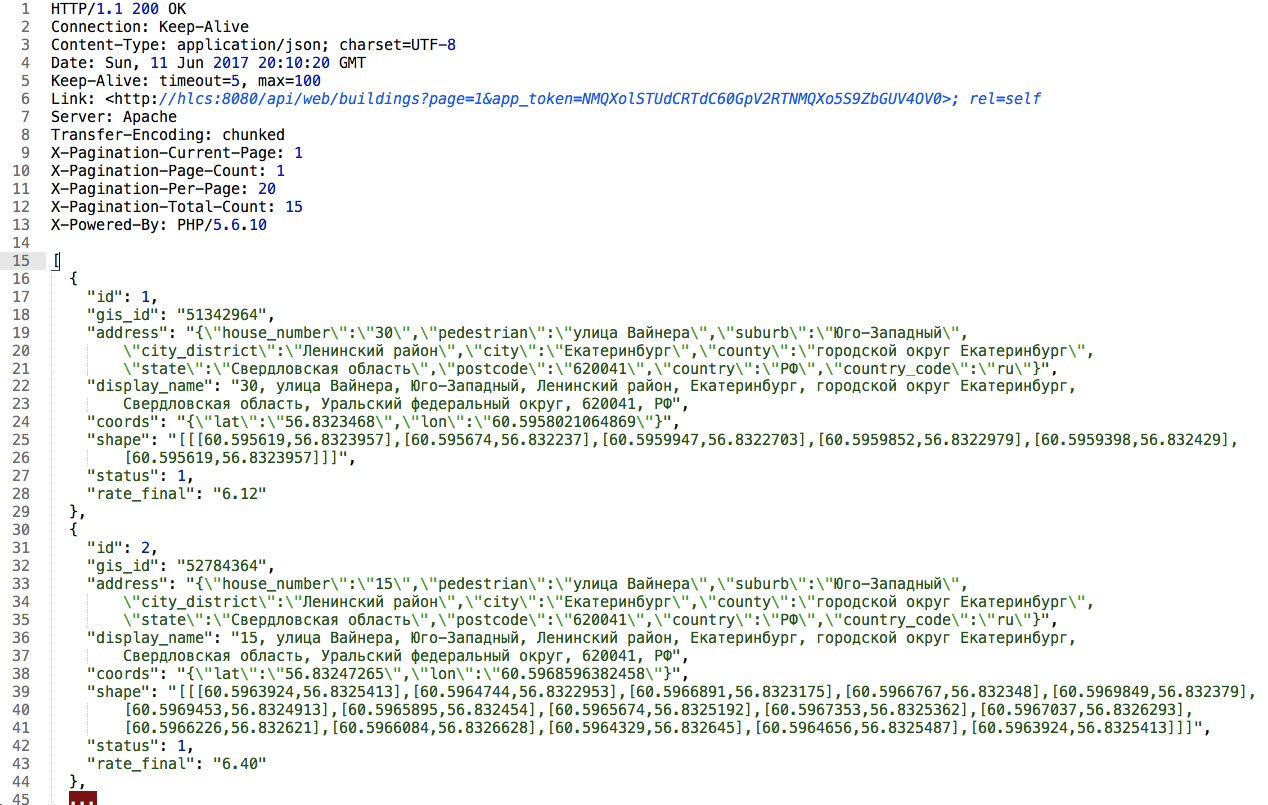
\includegraphics[width=1\textwidth]{images/queries/buildings_get_from}
		\caption{Ответ к запросу на получение списка зданий}
		\label{query:buildings_get_from}
	\end{figure}

	\begin{figure}[t!]
		\centering
		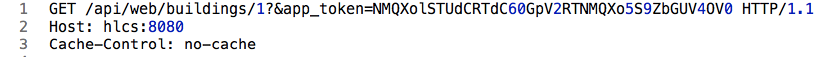
\includegraphics[width=0.9\textwidth]{images/queries/buildings_get_one_to}
		\caption{Пример запроса на получение информации о конкретном здании}
		\label{query:buildings_get_one_to}
	\end{figure}

	\begin{figure}[t!]
		\centering
		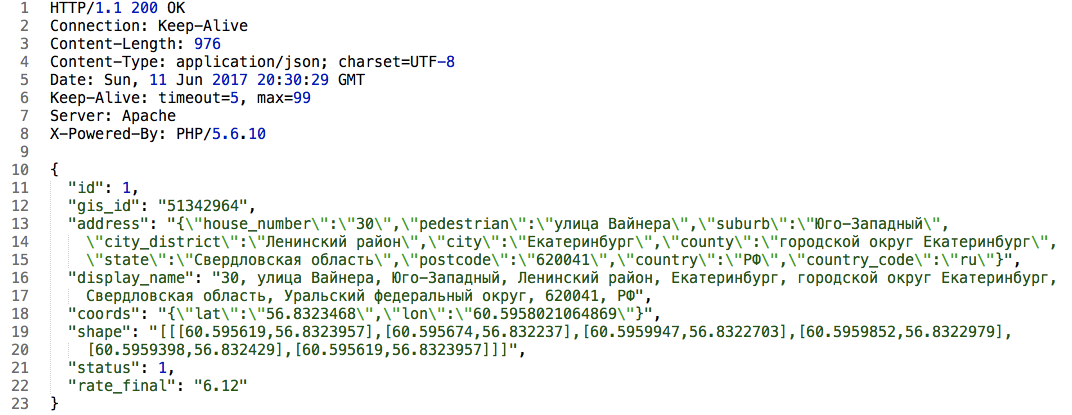
\includegraphics[width=1\textwidth]{images/queries/buildings_get_one_from}
		\caption{Ответ к запросу на получение информации о конкретном здании}
		\label{query:buildings_get_one_from}
	\end{figure}

\subsection{Экранные формы}

	Пользовательский интерфейс прототипа не содержит элементы доступа к функциям системы, предоставляемым API. В качестве альтернативы предлагаемое решение включает в себя реализацию пользовательского web-интерфейса САТУ, работающего как клиентское приложение, использующее API.
 
	Доступ к web-приложению осуществляется через браузер. Доступ к основным страницам осуществляется с помощью главного меню, расположенного в верхней части каждой web-страницы. Главная страница (рисунок \ref{scrshot:main_1}) поделена на две части: панель поиска зданий и интерактивная карта Google Maps. Здания, которые были проанализированы САТУ, выделяются цветом по шкале от красного до зелёного в соответствии с оценкой энергоэффективности.

	\begin{figure}[h!]
		\centering
		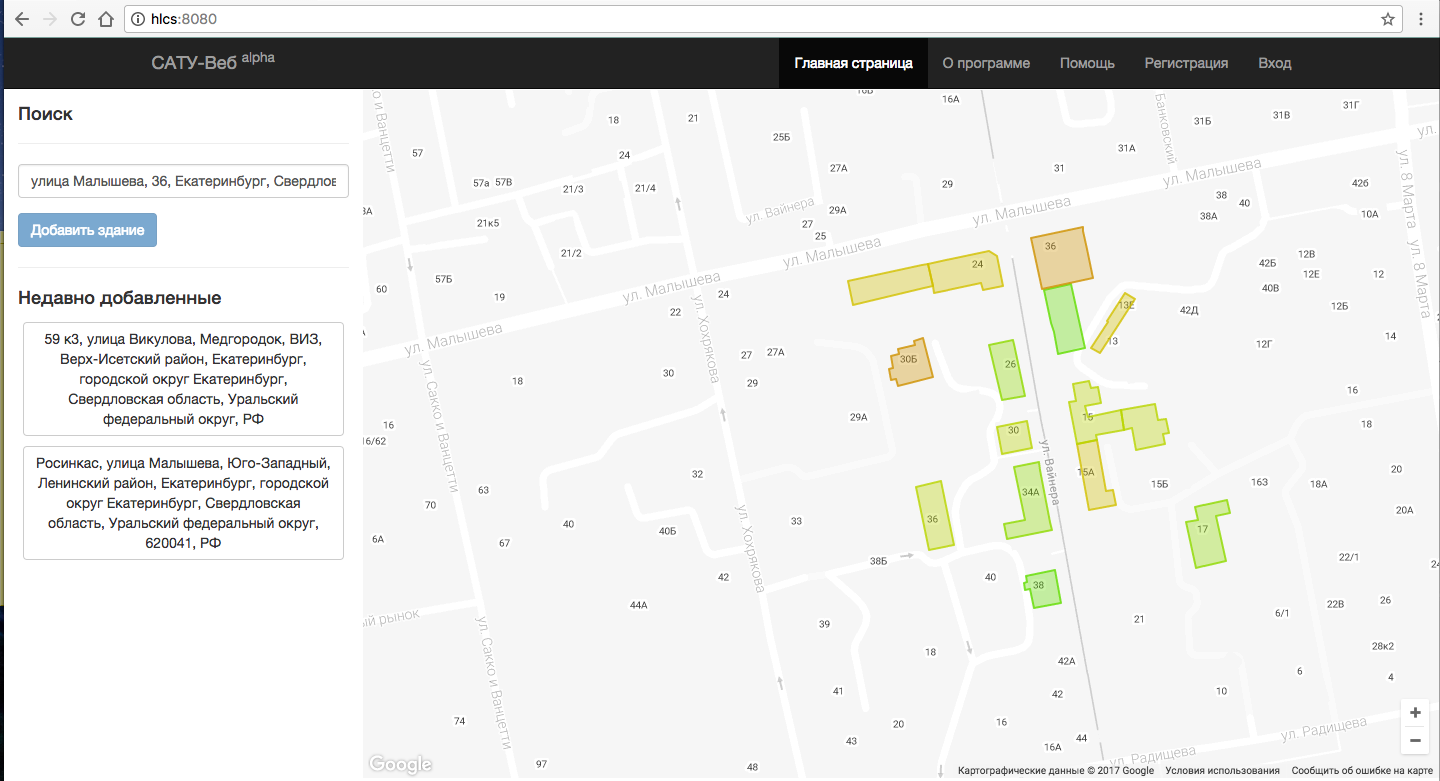
\includegraphics[width=0.9\textwidth]{images/scrshots/main_1}
		\caption{Главная страница веб-интерфейса САТУ}
		\label{scrshot:main_1}
	\end{figure}

	При введении пользователем интересующего адреса в поле поиска формируется выпадающий список (рисунок \ref{scrshot:search_field_1}) с доступными в ГИС адресами зданий.

	\pagebreak

	\begin{figure}[h!]
		\centering
		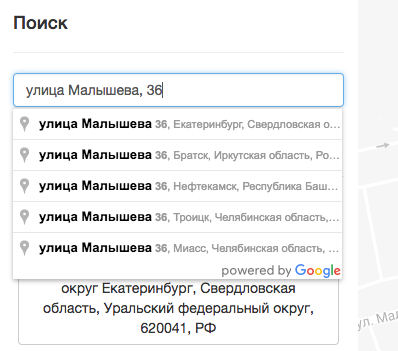
\includegraphics[width=0.4\textwidth]{images/scrshots/search_field_1}
		\caption{Процедура поиска здания с помощью Google Maps}
		\label{scrshot:search_field_1}
	\end{figure}

	После выбора адреса из списка возможно два варианта поведения: если здание найдено в САТУ, оно отобразится в центре карты; в противном случае здание дополнительно выделяется розовым цветом (рисунок \ref{scrshot:main_new_1}).

	\begin{figure}[h!]
		\centering
		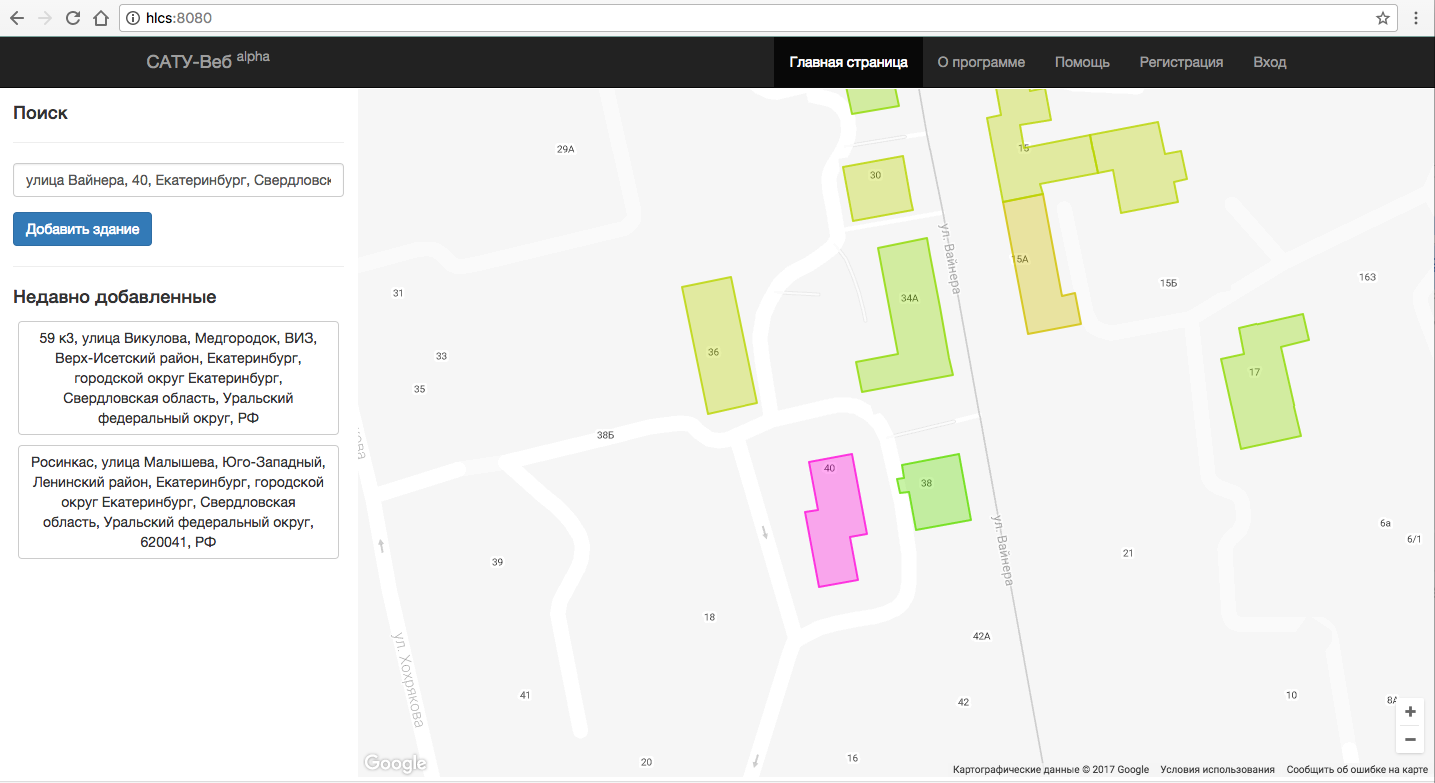
\includegraphics[width=0.9\textwidth]{images/scrshots/main_new_1}
		\caption{Отображение здания, не обнаруженного в САТУ}
		\label{scrshot:main_new_1}
	\end{figure}

	\pagebreak

	При нажатии левой кнопкой мыши по подсвеченному зданию на карте рядом с ним отображается всплывающее окно с краткой информацией и ссылкой на страницу с подробными сведениями (рисунок 4.12).

	\begin{figure}[h!]
		\centering
		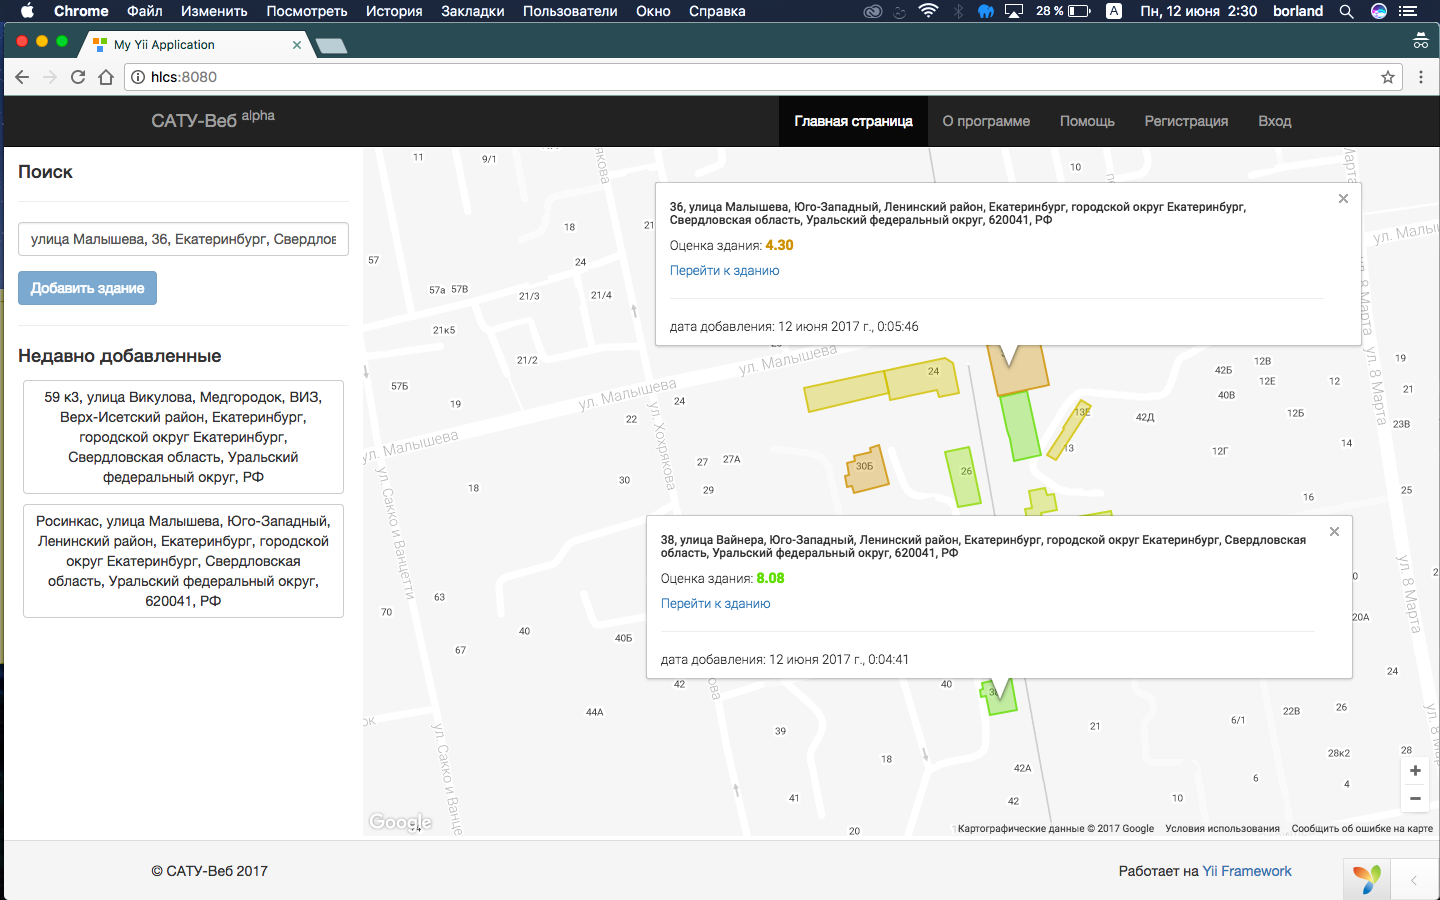
\includegraphics[width=0.9\textwidth]{images/scrshots/main_selected_1}
		\caption{Взаимодействие с проанализированными зданиями на карте: отображение всплывающих окон}
		\label{scrshot:main_selected_1}
	\end{figure}

	В случае, если здание выделено розовым цветом, в панели поиска становится доступна кнопка “Добавить здание”. При нажатии на неё пользователь перейдёт на страницу “Добавить/изменить здание” (рисунок \ref{scrshot:update_1}). Эта страница позволяет просмотреть историю съёмки здания. При необходимости пользователь может добавить новую серию снимков, нажав на кнопку “Добавить серию снимков”.

	\pagebreak

	\begin{figure}[t!]
		\centering
		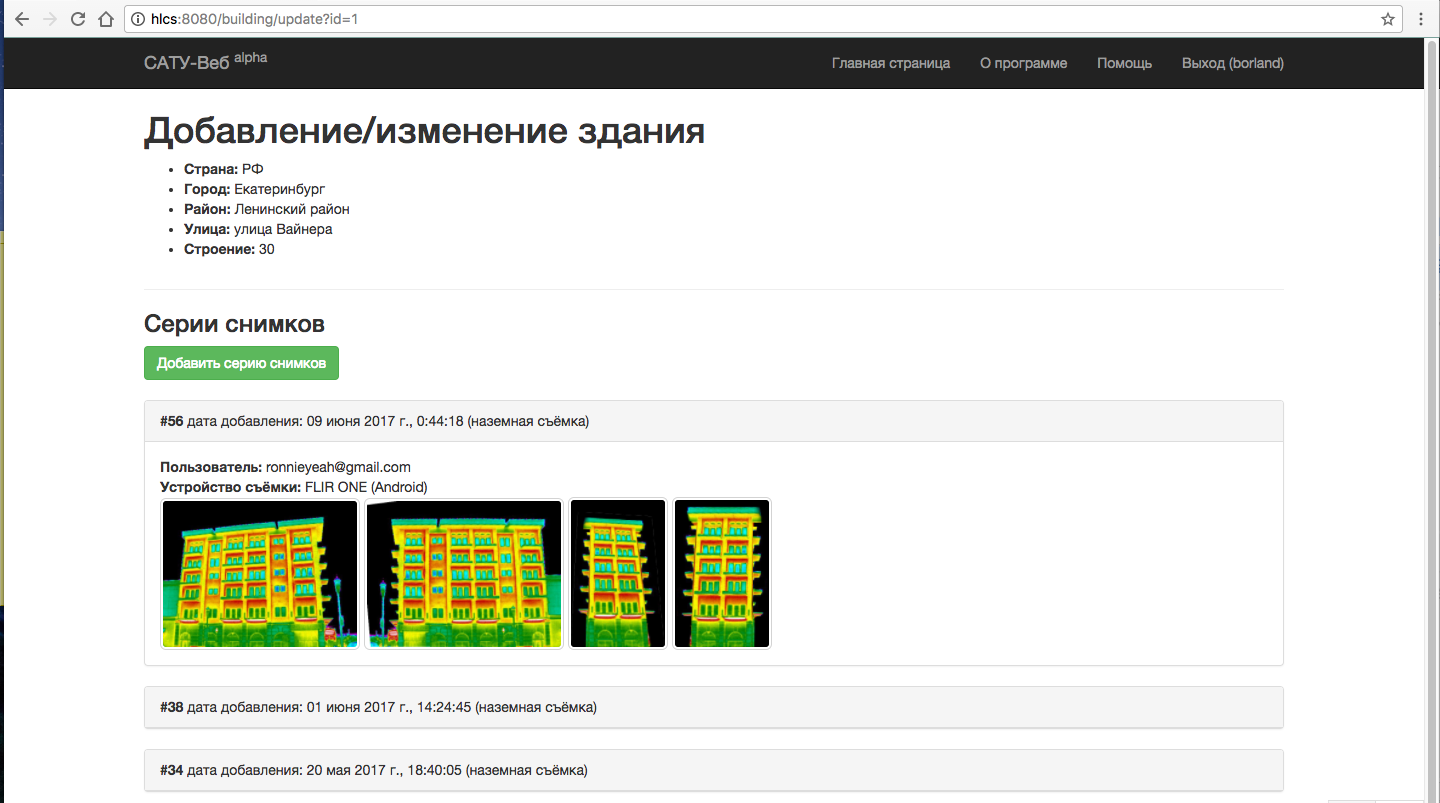
\includegraphics[width=0.9\textwidth]{images/scrshots/update_1}
		\caption{Форма добавления/изменения здания}
		\label{scrshot:update_1}
	\end{figure}

	Загрузка серии снимков через web-приложение в браузере проходит в два этапа: 

	\begin{itemize}
		\item выбор типа, устройства съёмки, непосредственно загрузка ИК изображений (рисунок \ref{scrshot:add-series_1});
		\item указание дополнительных данных о загруженных снимках (положение камеры) (рисунок \ref{scrshot:add-series_2}).
	\end{itemize}
 
	Форма загрузки изображений использует два способа выбора файлов: перетаскивание в область формы вручную; указание каталога вручную при нажатии на кнопку "Выбрать". После выбора в форме отображаются пиктограммы изображений и указывается их размер. При желании изображения можно удалить из формы.

	\pagebreak

	\begin{figure}[t!]
		\centering
		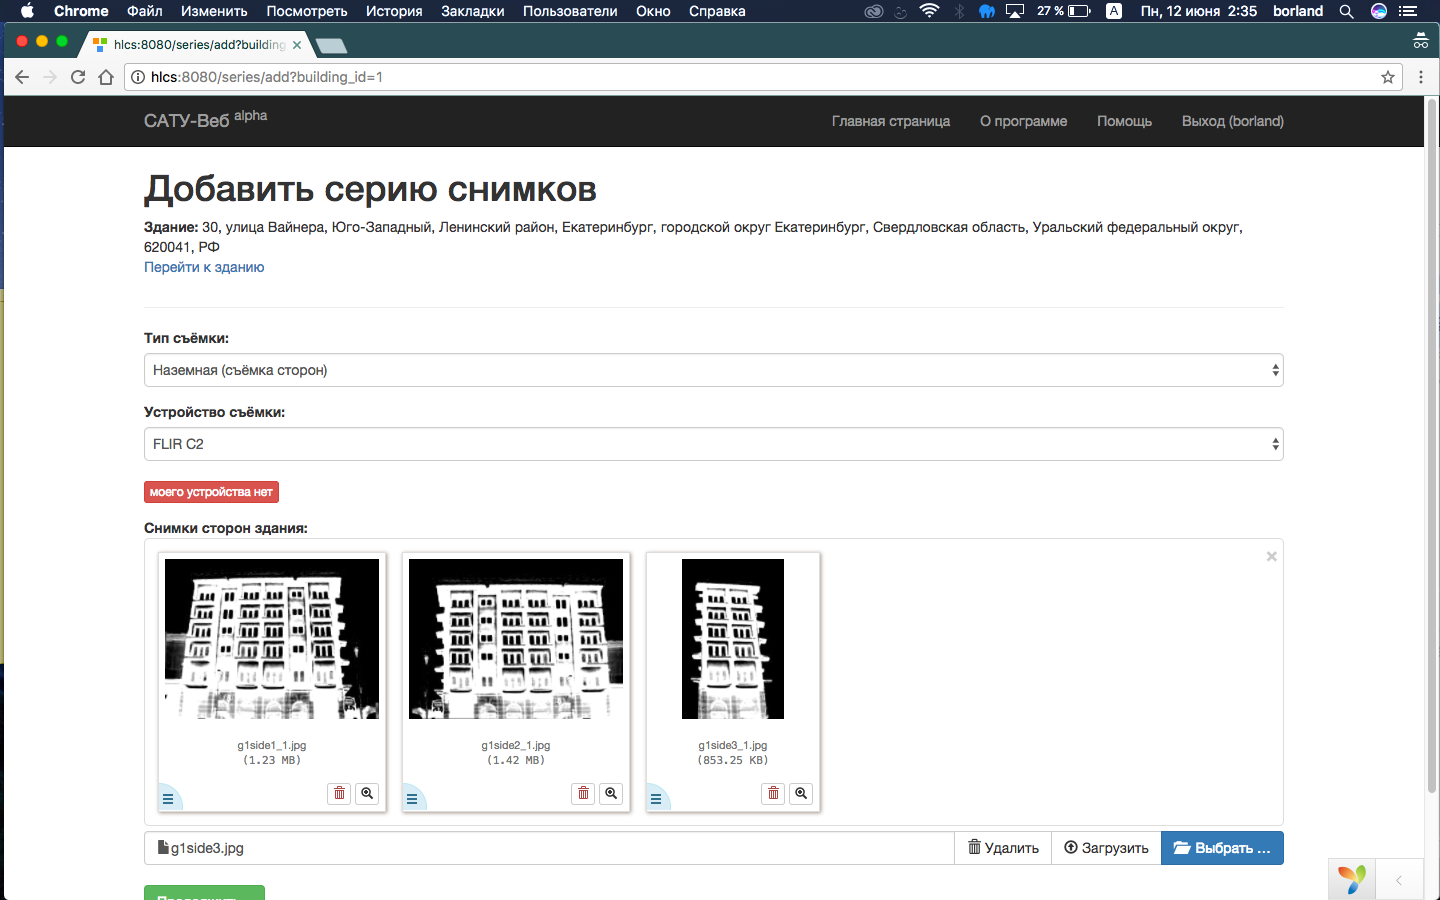
\includegraphics[width=0.9\textwidth]{images/scrshots/add-series_1}
		\caption{Форма добавления серии снимков (этап 1)}
		\label{scrshot:add-series_1}
	\end{figure}

	\begin{figure}[h!]
		\centering
		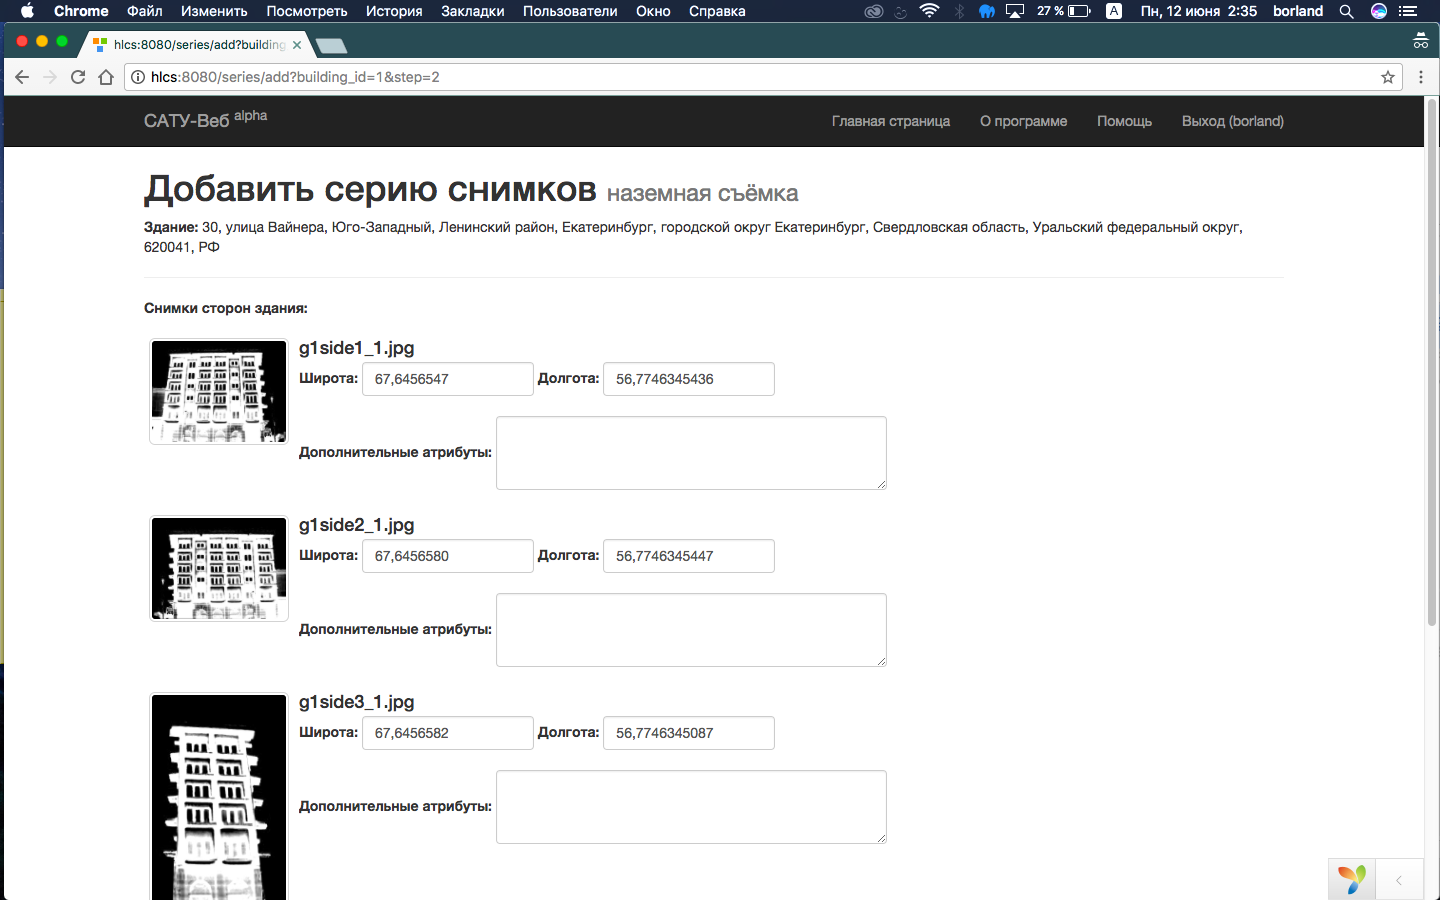
\includegraphics[width=0.9\textwidth]{images/scrshots/add-series_2}
		\caption{Форма добавления серии снимков (этап 2)}
		\label{scrshot:add-series_2}
	\end{figure}

	\pagebreak

	После успешного добавления здания в САТУ на главной странице в разделе “Недавно добавленные” отображаются последние зарегистрированные системой здания. При нажатии на кнопку с адресом здания карта мгновенно переносит обзор на него.
 
	Некоторые действия, такие как загрузка снимков и добавление зданий, недоступны пользователям, не представившимся в системе. Для этого предусмотрены страницы с формами регистрации и входа в систему (рисунки \ref{scrshot:register_1}, \ref{scrshot:login_1}).

	\begin{figure}[h!]
		\centering
		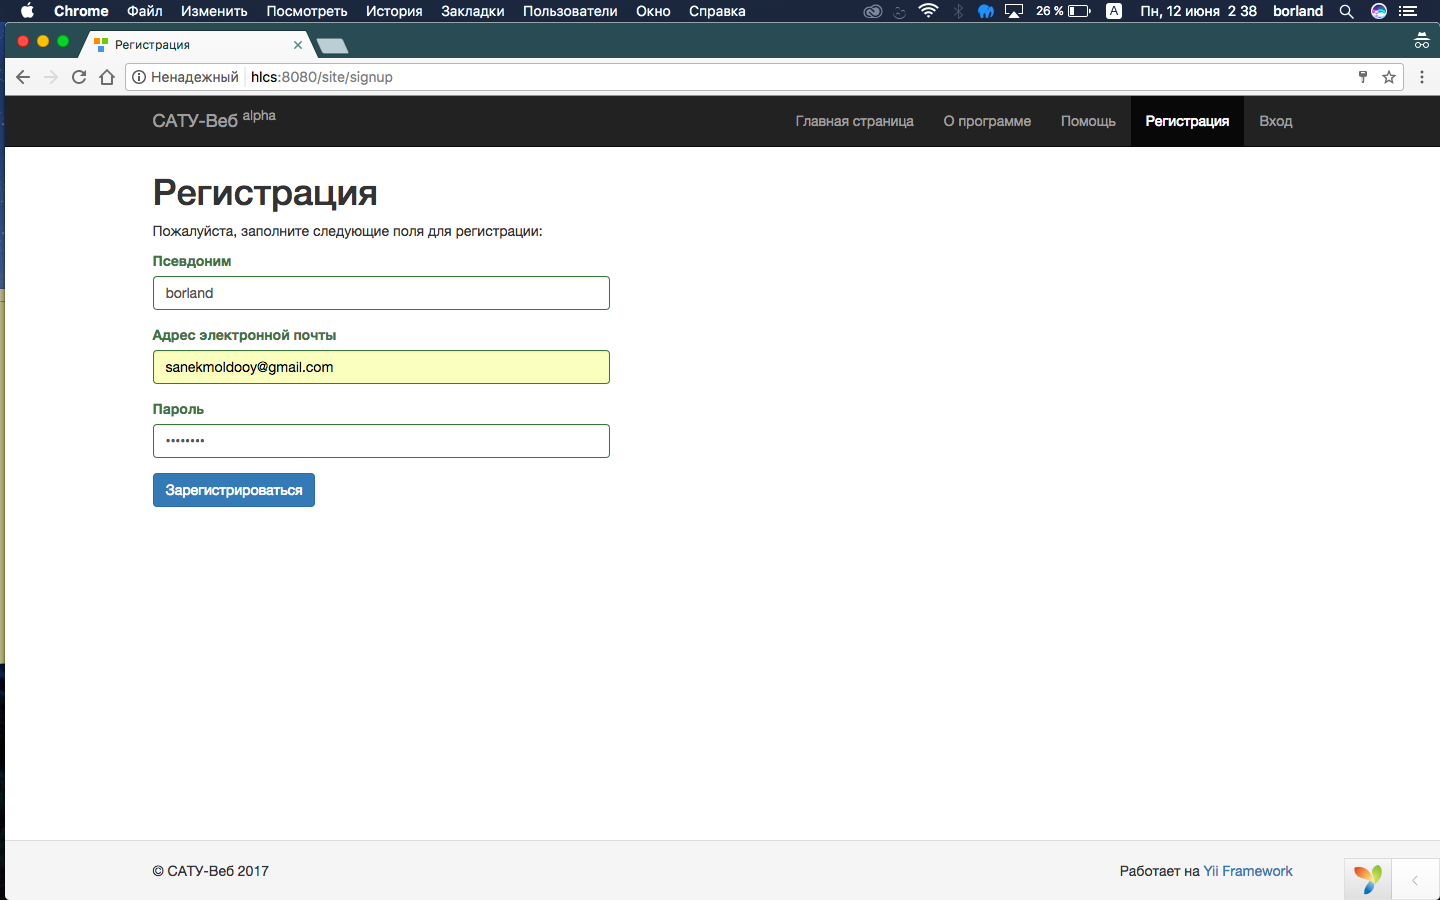
\includegraphics[width=0.5\textwidth]{images/scrshots/register_1}
		\caption{Форма регистрации в системе}
		\label{scrshot:register_1}
	\end{figure}

	\begin{figure}[h!]
		\centering
		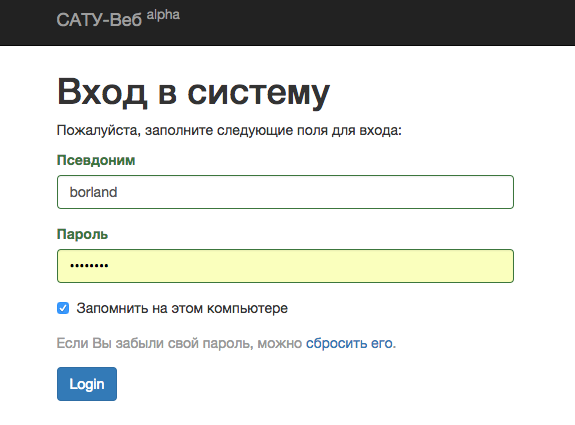
\includegraphics[width=0.5\textwidth]{images/scrshots/login_1}
		\caption{Форма входа в систему}
		\label{scrshot:login_1}
	\end{figure}

	\pagebreak

\section{Результаты и выводы по главе 4}

\par

	По завершении этапа инженерной реализации разрабатываемого программного интерфейса были получены следующие результаты:

	\begin{itemize}
		\item на основе выдвинутых в главе \ref{chap:design} архитектурных решений реализована база данных с помощью пакета MySQL Workbench и разработан каркас для программного кода API на базе платформы Yii2 Framework;
		\item выполнена программная реализация функций обработки входящих запросов, произведены их тестирование и отладка;
		\item приведены примеры основных запросов и возможных ответов реализованного продукта;
спроектированы экранные формы клиентского web-приложения, работающего по реализованному программному интерфейсу.
	\end{itemize}
	
	\textbf{Выводы}: программный интерфейс, работающий в составе САТУ, способен интегрировать в систему клиентские приложения с помощью Интернет, независимо от операционной системы и программных платформ, на которых они работают эти приложения. Итоговый вариант реализации соответствует требованиям, установленным в Техническом задании на разработку программного интерфейса (приложение \ref{app-tz}).


